\documentclass[preprint,12pt,authoryear]{elsarticle}
\usepackage[T1]{fontenc}
\usepackage[utf8]{inputenc}
\usepackage{mathptmx}
\usepackage[expansion=false]{microtype}
\usepackage{booktabs}
\usepackage{tabularx}
\usepackage{enumitem}
\usepackage{xcolor}
\usepackage{tikz}
\usetikzlibrary{arrows.meta,positioning}
\usepackage[hidelinks]{hyperref}
\usepackage{lineno}
\setlist{itemsep=2pt,topsep=4pt}
\newcolumntype{L}{>{\raggedright\arraybackslash}X}
\renewcommand{\arraystretch}{1.15}
\setlength{\emergencystretch}{3em}
\newcommand{\code}[1]{\texttt{#1}}
\newcommand{\priv}{\textsuperscript{\textdagger}}
\journal{Journal of Systems and Software}

\begin{document}
\begin{frontmatter}
\title{Records Outsiders Can Recheck: Verifying the Verifiers of an Open Evidence Stack for AI Agent Actions in Production}
\author{Toshikatsu Oga\corref{cor1}}
\ead{contact@the-horizons-innovation.com}
\cortext[cor1]{Corresponding author. ORCID 0009-0000-9180-903X.}
\affiliation{organization={The HORIZONs Co., Ltd.},
  addressline={Win Aoyama 942, 2-2-15 Minami-Aoyama, Minato-ku},
  city={Tokyo},
  postcode={107-0062},
  country={Japan}}

\begin{abstract}
We report on an open stack that records what AI agents were authorized to do and what they did as signed canonical records in a public ledger anchored to Bitcoin, settles two-party contracts by an offline function, and records detected drift and authorized repair. Its central requirement is that a party outside the operator, using only public software, reaches the same verdict as the operator. We ask how far that requirement holds and what checking it finds. Over 83 days of production (22 July to 13 October 2026) we combined six methods: frozen corpora compared by verdict signature, a specification-only reimplementation by fenced AI agents, reimplementation by outside developers, cross-language differential testing, mutation analysis of the corpora, and a nightly board that reruns outside implementations from their own repositories. The specification-only reimplementation matched 13 of 18 verdicts before a normative verifier text existed and 18 of 18 after. Two outside developers, both with working relationships with the project, wrote three verifiers from the specification; on the last board run all implementations reproduced every expectation and five agreed on 40 freshly signed bundles. The frozen corpora detected only 5 of 13 faults we declared; eight new vectors detect all 13. Operation found defects no test had caught, including a ledger sequencing race that leaves the hash chain intact while replacing an entry. No unaffiliated party uses the stack in production yet, and the repair layer's witness quorum has never been met; we report these as measured zeros.
\end{abstract}

\begin{keyword}
AI agents \sep Verifiable records \sep Conformance testing \sep Mutation analysis \sep Differential testing \sep Specification ambiguity \sep Experience report
\end{keyword}
\end{frontmatter}

\linenumbers

\section{Introduction}

An AI agent that books a service, edits a file in someone else's repository or delegates a subtask to another agent leaves a trail of claims: who authorized what, what was executed and what the result was. Those claims are usually written by the system that acted, stored where it chooses and, if summarized, turned into a score that whoever publishes it can tune.

This paper reports on an attempt to produce records of agent actions whose verification does not require trusting their producer. Each record is a set of canonical bytes signed by the party who asserts it, batched into a public ledger whose head is anchored to Bitcoin, and checked by an offline verifier that anyone can install. The verifier returns evidence and lists what that evidence does not establish; it does not return a score or make a decision.

Two difficulties dominate. A record is only as checkable as the specification that defines it: if a careful reader of the specification would compute a different verdict, the record is in practice checked against the author's program, not against a public rule. And a verifier's corpus of test fixtures is written by the same people who wrote the verifier, so passing it says less than it appears to. Most of this paper measures, and reduces, these two gaps on a system that was in production while we measured it.

\subsection{Industrial setting}\label{sec:setting}

The work was carried out at The HORIZONs Co., Ltd., a small company in Tokyo that operates HORIZON SHIELD, a buyer-side service that checks construction and renovation quotes in Japan against public cost data. The service exposes its checks as tools that AI agents call through the Model Context Protocol, and agents increasingly called them on behalf of people who were not our customers. The question that started the work was practical: when an agent cites one of our fair-price receipts, or another agent claims to have called us, how can a third party check that claim without trusting us? The stack described here grew from that question between July and October 2026.

The setting shaped the result. One person operates production; code, audits and deployment scripts are prepared with an AI assistant, and every push, deployment and secret operation is done by hand by that person. Production runs on Cloudflare Workers with an eventually consistent key-value store, GitHub Actions and a few jobs on the operator's own machine. The budget was small, so every outside check had to be free to run: public repositories, public packages and Bitcoin as the only shared clock. The events reported below, including the defects, happened in that production setting, not in a laboratory.

\paragraph{Research questions}
\begin{description}[leftmargin=3.2em,style=nextline]
\item[RQ1] How far does the specification alone determine the verdict? (Section~\ref{sec:rq1})
\item[RQ2] How well do the frozen corpora separate a correct verifier from a faulty one? (Section~\ref{sec:rq2})
\item[RQ3] Do implementations by other developers agree with the reference, and keep agreeing over time and on unseen inputs? (Section~\ref{sec:rq3})
\item[RQ4] What does operating the stack find that the tests did not? (Section~\ref{sec:rq4})
\end{description}

\paragraph{Contributions} (i) A combination of six verification methods applied to the verifiers of a records system, including a repeatable specification-only reimplementation by fenced AI agents and mutation analysis of conformance corpora rather than of a program's own tests (Section~\ref{sec:design}). (ii) Measurements from 83 days of production that separate the operator's own tooling from named outside parties and state each party's relationship to the project (Section~\ref{sec:results}). (iii) A catalogue of defects found after the tests passed, with their mechanisms (Section~\ref{sec:rq4}). (iv) The indicators on which nothing has happened yet (Section~\ref{sec:zeros}).

The architecture is described only as far as the results need it (Section~\ref{sec:system}). The system is a recombination of known components and we claim no novelty for it.

\section{Background and related work}\label{sec:related}

\paragraph{Tamper-evident logs} Secure audit logs~\citep{schneier1999}, tamper-evident logging structures~\citep{crosby2009}, Certificate Transparency~\citep{rfc6962}, key transparency~\citep{coniks} and Sigstore's Rekor~\citep{sigstore} publish append-only records that third parties can audit. Linking timestamps goes back to Haber and Stornetta~\citep{haber1991}; OpenTimestamps~\citep{ots} commits a hash to a Bitcoin~\citep{nakamoto2008} transaction so that its existence before a block can be checked without the timestamping service. Our ledger uses these ideas; what differs is the subject of the records and the requirement that each verdict also be re-derivable by a second implementation.

\paragraph{Provenance and supply chains} The in-toto framework~\citep{intoto}, SLSA~\citep{slsa}, TUF~\citep{tuf} and W3C PROV~\citep{prov} record who did what to which inputs; reproducible builds~\citep{lamb2022} require byte-identical artifacts from independent builds. Software Heritage~\citep{swh} preserves source code outside its authors' control; our recovery drill uses it.

\paragraph{Identity, canonical form and signatures} We use Ed25519~\citep{bernstein2012,rfc8032} keys as \code{did:key} identifiers~\citep{didcore,didkey} and a canonical JSON form close to RFC 8785~\citep{rfc8785}. The divergence of Ed25519 verifiers on small-order and mixed-order keys is documented~\citep{chalkias2020,brendel2021}; Section~\ref{sec:rq4} reports that our first verifier had exactly this gap.

\paragraph{Agent protocols and accountability} The Model Context Protocol~\citep{mcp} and the Agent2Agent protocol~\citep{a2a} define how agents discover and call tools and each other. Agent payment mandates~\citep{ap2} and OAuth rich authorization requests~\citep{rfc9396} carry signed or structured authorizations; visibility into agent activity has been argued for as an accountability measure~\citep{chan2024}. Our records are complementary: they bind an authorization, an execution report and outside observations into one verdict that a second implementation can recompute. We report interoperability exercises with three open projects in this space: VATE~\citep{vate}, TRACE~\citep{trace} and PriorSeal~\citep{priorseal}.

\paragraph{Testing the tests} Mutation analysis~\citep{demillo1978,jia2011,papadakis2019} measures whether tests distinguish a program from faulty variants, with known limits on how well mutants stand for real faults~\citep{just2014}. Differential testing~\citep{mckeeman1998,yang2011} compares implementations on the same inputs. Knight and Leveson~\citep{knight1986} showed that independently written versions fail together more often than independence predicts, which bounds what agreement between implementations can show. We apply these techniques to conformance corpora and to the verifiers that consume them.

\paragraph{Concurrency and error handling} Application-level read-modify-write without database support is common and error-prone~\citep{bailis2015}, the more so on eventually consistent stores~\citep{vogels2009,cfkv}. Most critical production failures trace to mishandled errors~\citep{yuan2014}. Both patterns appear in Section~\ref{sec:rq4}.

\paragraph{Prior work by the author} A working paper~\citep{ssrn7419998} tested one layer of the stack (monthly bundles of measured history) with one reimplementation by its co-author, written from the specification and the published files; the specification named 11 of a bundle's 20 fields. A peer-reviewed technical note~\citep{oga2026iic} measured the spread of construction cost figures in consumer-facing AI answers and argued for a verifiable reference layer. This paper covers the whole stack, adds five verification methods and reports production operation.

\section{The system in brief}\label{sec:system}

Table~\ref{tab:gloss} glosses the component names. All components share one canonical form (keys sorted by code point, integers within $\pm(2^{53}-1)$, printable ASCII keys, no Unicode normalization), SHA-256 in lowercase hexadecimal, Ed25519 keys as \code{did:key} identifiers or served at a party's own domain, and raw 64-byte signatures in standard padded base64, without a JSON Web Signature layer. A content identifier is the hash of the canonical preimage without signature fields; a signature covers the same preimage. Reimplementation is correspondingly small: the reference verifier is about 1,200 lines of JavaScript, its same-author Python port about 1,100 lines and one outside Python verifier about 800 lines.

\begin{table}[t]
\centering
\caption{Components and their production status on 13 October 2026.}
\label{tab:gloss}
\small
\begin{tabularx}{\textwidth}{@{}l L L@{}}
\toprule
Name & What it is & Status \\
\midrule
Ledger & Public append-only store; daily batches; hash chain with end marker since 28 Sep; OpenTimestamps stamping hourly & Live; 95 entries; stamping partly on the operator's machine \\
NENRIN & Signed evidence of delegation (witness observations), authorization (grant), execution (receipt) and intent; offline verifier & Live; verifier on npm and PyPI, Go port \\
MUSUBI & Two-party signed contracts; settlement is an offline function over executions, anchoring proofs and self-verified Bitcoin headers & Live intake; settlement v1 to v1.15 as code \\
SEKI & A relying party's signed admit or refuse decision before an act & Live demonstration; all parties are the operator \\
TSUGI & Hash-linked drift, proposal, signed authorization, execution and verification records; witnesses drawn by lottery from a Bitcoin block & Live verifier; quorum never met \\
TSUNAGI & Nightly board that reruns registered implementations from their own repositories & Live; 12 implementations, 7 by outside authors \\
Gate & Daily measurement of public agent endpoints at coordinates derived from a committed salt and a later Bitcoin block & Live; most outside walkers measure it \\
\bottomrule
\end{tabularx}
\end{table}

\paragraph{Ledger} Each entry commits to a \code{claim\_sha256}. The hash of entry $n$ covers its number, schema, claim hash, creation time and the hash of entry $n-1$; entry 1 links to 64 zeros; an end marker binds the head so that dropping the newest entries is visible in the export alone. We added the chain after scoring our export with the checker of an outside specification, VLC-1~\citep{vlc1}, which rated it at its lowest level because no entry bound its predecessor. A daily job batches pending submissions; each batch carries the current head inside its anchored bytes.

\paragraph{NENRIN} A provenance bundle for one task contains witness observations (one delegation hop, signed by an observer and by the delegating party), a grant (action, caller, provider, validity window; signed by the caller), a receipt (executed action, outcome digest, time; signed by the provider) and optionally an intent. The verifier checks the delegation chain, the execution (action match, one reconciled outcome, receipt bound to grant, executor authorized), preflight and evidence links. Its output's \emph{verdict signature} is the triple of verdict, set of refusal codes and set of finding codes; there are 14 refusal and 9 finding codes. Each report also lists six things it does not establish, beginning with ``that any executed action occurred in the world''. The normative text is archived~\citep{zenodoverifier}. Separately, \emph{witness walks} record what a service's public endpoints returned to an outside walker, signed under a key served at the walker's domain; the ledger refuses a walk whose key is served by the walked host or by the ledger.

\paragraph{MUSUBI and SEKI} A contract lists authorized, prohibited and conditional actions, witnesses, approvers, limits and a finality depth, and is identified by the hash of its canonical bytes. Executions name that hash. Settlement takes the contract, the executions with their anchoring proofs and Bitcoin headers the settler verified itself, and returns a verdict such as \code{within\_grant} and \code{final}. Sixteen versions (v1 to v1.15) were published; most revisions followed a finding by a public red team, the counterparty or our own review, the rest added features. SEKI admission records let a relying party sign its decision before an act; the ledger stores and anchors them and renders no decision.

\paragraph{TSUGI} Repairs are drawn from a closed catalogue and authorized by the operator key. Verification witnesses are drawn with a seed hashed from a Bitcoin block hash, the pool hash and the subject hash; the subject is anchored before the beacon block exists, so a witness cannot choose the draw and the operator can influence it only by appending extra commitments before the beacon block, which the ledger would show. When a quorum is required and not met, the verifier withholds the recovery claim and reports \code{witness\_quorum\_short}.

\paragraph{TSUNAGI} Each night the board clones each registered implementation at its latest commit and runs it on the frozen corpora. A cell is \emph{board-scored} when the board feeds fixtures and compares outputs itself, and \emph{self-scored} when it repeats the implementation's own count. The board also signs 40 fresh adversarial bundles with new keys each night; implementations that accept batch input must agree on all of them.

\begin{figure}[t]
\centering
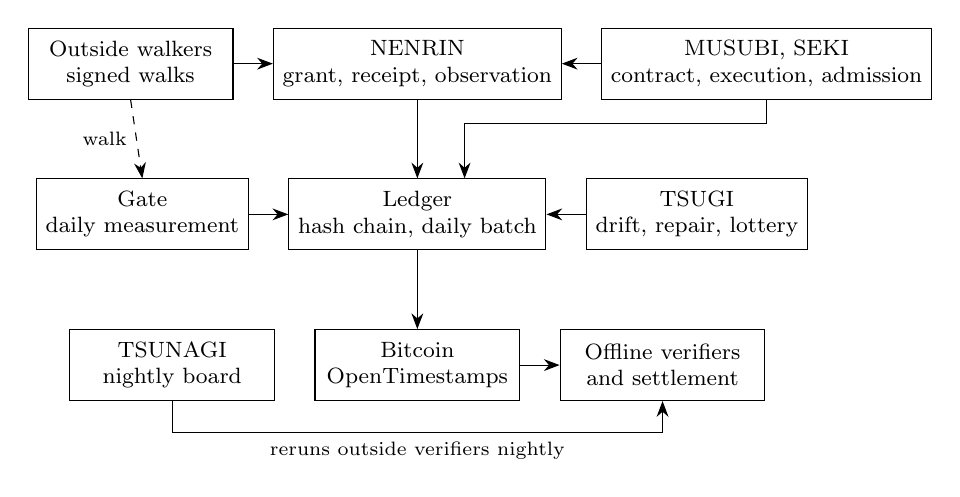
\begin{tikzpicture}[node distance=6mm and 5mm, every node/.style={font=\footnotesize}, box/.style={draw, minimum width=26mm, minimum height=9mm, align=center}, arr/.style={-{Stealth[length=2mm]}}]
\node[box] (walk) {Outside walkers\\signed walks};
\node[box, right=of walk] (nen) {NENRIN\\grant, receipt, observation};
\node[box, right=of nen] (mus) {MUSUBI, SEKI\\contract, execution, admission};
\node[box, below=10mm of nen] (led) {Ledger\\hash chain, daily batch};
\node[box, left=of led] (gate) {Gate\\daily measurement};
\node[box, right=of led] (tsugi) {TSUGI\\drift, repair, lottery};
\node[box, below=10mm of led] (btc) {Bitcoin\\OpenTimestamps};
\node[box, right=of btc] (ver) {Offline verifiers\\and settlement};
\node[box, left=of btc] (board) {TSUNAGI\\nightly board};
\draw[arr] (walk) -- (nen);
\draw[arr] (mus) -- (nen);
\draw[arr] (nen) -- (led);
\draw[arr] (mus.south) -- ++(0,-3mm) -| ([xshift=6mm]led.north);
\draw[arr] (gate) -- (led);
\draw[arr] (tsugi) -- (led);
\draw[arr] (led) -- (btc);
\draw[arr] (btc) -- (ver);
\draw[arr] (board.south) -- ++(0,-4mm) -| node[pos=0.25, below, font=\scriptsize]{reruns outside verifiers nightly} (ver.south);
\draw[arr, dashed] (walk.south) -- node[left, font=\scriptsize]{walk} (gate.north);
\end{tikzpicture}
\caption{Data flow as built. Records are signed by the asserting party, batched into the ledger and anchored. Verification and settlement run offline from published code; the board reruns outside implementations against corpora derived from these layers. Outside walkers mostly measure the gate. The diagram was drawn as TikZ code written with the assistance of a generative AI tool and checked by the author.}
\label{fig:flow}
\end{figure}

\section{Study design}\label{sec:design}

\paragraph{Terms} We call a party \emph{outside} if it is not employed by or under the control of the operator. Outside is not \emph{independent}: no outside implementer or witness in this paper is unaffiliated with the project. babyblueviper1 co-authored earlier work on this stack~\citep{ssrn7419998} and is the counterparty in two MUSUBI contracts; kuangmi-bit contributed two corpora to the repository and is a party to a MUSUBI contract; astrogilda contributed two pull requests; the author reviewed a project by pipavlo82. Only luiksksk, Agenstry and the official A2A Python SDK have no other recorded relationship. A \emph{reproduction} reruns our published tool; an \emph{implementation} is the party's own code. Ports written by the author are reported and never counted as independent.

\paragraph{Methods} Each method answers a different part of the question \emph{would a careful outside reader of the public text compute the same verdict?}
\begin{enumerate}[label=M\arabic*.]
\item \textbf{Frozen corpora by verdict signature} (RQ2, RQ3). Expectations compare the verdict and the sets of codes, never the reasons. A corpus, once published, is never edited; new fixtures go into a new corpus.
\item \textbf{Specification-only reimplementation} (RQ1). A fresh AI agent receives the specification text and the fixture bundles, but neither the code nor the expected results nor network access, and writes a verifier; the operator scores its output afterwards. The fence makes the experiment repeatable after each specification change.
\item \textbf{Outside reimplementation} (RQ1, RQ3). Developers outside the project write verifiers in their own repositories and languages.
\item \textbf{Cross-language differential testing} (RQ3). The reference and the author's ports run on large sets of mutated inputs; a pair agrees if both throw, or if both give the same verdict signature and the same ordered list of codes and reasons.
\item \textbf{Mutation analysis of the corpora} (RQ2). We declare faults as single exact substitutions in the verifier and ask whether any frozen fixture changes its verdict signature. We used an independently published tool, corpus-adequacy~0.8.0~\citep{corpusadequacy}, and cross-checked it with our own script.
\item \textbf{Nightly board} (RQ3). Outside implementations are rerun from their authors' repositories every night, on the frozen corpora and on 40 fresh adversarial bundles.
\end{enumerate}

\paragraph{Data} Unless marked, every number below can be traced to a file, commit or ledger entry in the public repository~\citep{repo}. Numbers marked \priv{} come from the operator's log or from the specification-only reimplementation transcripts, which are released with the replication package~\citep{replication}.

\section{Results}\label{sec:results}

\subsection{Ledger state}\label{sec:ledger}

On 13 October 2026 the ledger head reported $n=95$ with an intact chain\priv. A public snapshot of entries 1 to 88, taken on 12 October, allowed an offline recomputation of the whole chain and the end marker; both matched the stored head. Each of the 88 entries carries a recorded OpenTimestamps attestation with a Bitcoin block height and a proof file; the first entry dates from 22 July 2026 (block 959118). We did not re-verify the proofs against Bitcoin headers for this paper. The newest entries were awaiting their stamps at the time of writing.

A scheduled drill rebuilt the ledger 28 times between 30 September and 12 October from two copies: a GitHub copy that the operator controls (14 of 14 runs rebuilt it; this shows the copy's form, not its survival) and a Software Heritage copy that the operator does not host (9 runs rebuilt it; 5 found the archive unavailable, including the last four).

Three outside domains have signed walks in the ledger under keys served at their own domains: \code{api.babyblueviper.com} (entries 57 and 61), \code{pipavlo82.github.io} (entries 65 and 73) and \code{kuangmi-bit.github.io} (twelve records in entries 71 to 84, from a repository created from our witness template). Two of the three are GitHub Pages subdomains rather than registered domains, and all three parties have working relationships with the project. Many other batches are walks by the operator's own runners and are labelled as such.

\subsection{RQ1: How far does the specification determine the verdict?}\label{sec:rq1}

\paragraph{Specification-only rounds} In the first round (4 October 2026) a fenced agent received the delegation and execution specifications, the provenance overview and 18 fixture bundles. It reproduced the cryptographic core at once (canonical form, four content identifiers, five signature types, \code{did:key}) but matched only 13 of 18 verdict signatures\priv. It recorded eleven independent guesses, each of which moved at least one verdict; whether findings are reported on refused reports alone moved 11 of 18\priv. The bundle format and the intent record were not defined, and several files the text cited as normative, among them the canonical vectors, were not available to the implementer.

We then wrote a single normative verifier text and fixed the errors the agent had found. A new agent, given that text, the specifications, the canonical vectors and the same 18 bundles, matched 18 of 18 signatures and 9 of 9 canonical vectors and recorded no guess that affected a bundle\priv; the comparison with the withheld expectations was made afterwards. The second round still listed gaps outside the corpus (absent versus null, lexical forms of numbers, regular-expression and base64 flavours) and found that the provenance overview contradicted the verifier text on the evidence target, which would change two signatures. Several of these gaps later became rules. Both agents were of the model family that had assisted in writing the specification and the reference, so common-mode readings cannot be excluded (Section~\ref{sec:threats}).

\paragraph{Outside implementations} The first outside verifier, by kuangmi-bit, was written in Python from the specification text before the normative verifier text existed. It matched 5 of 5 verdicts and all 21 digests, and its author reported five specification gaps (signature input, the scope of one rule, reasons versus codes, undefined findings, the linkage rule), which we fixed in a new corpus. The same author's second verifier, written from the normative text, matched 18 of 18; the new edge-case rules exposed two bugs in its own code. The author's earlier implementation had scored 8 of 18 against the corpus that followed the five fixes. A third verifier, by babyblueviper1, is declared by its author to have been written from the normative text alone; we cannot check that fence, and its author had worked with our code before.

\paragraph{Answer to RQ1} For this specification, the text as first published left about a quarter of verdicts to the implementer's guesses; one normative text closed the gaps that the corpus exercises, but each new reader, human or agent, has found further gaps outside it.

\subsection{RQ2: How well do the corpora separate faulty verifiers?}\label{sec:rq2}

We declared 13 faults in the Python port, each a single exact substitution (for example, the grant signature check always succeeds, or the upper bound of the validity window is ignored), plus a positive control (every refusal dropped) and an inert control. The controls behaved: the positive control changed 63 fixtures, the inert control none. The 93 fixtures of the five frozen corpora detected 5 of the 13 faults (score 38.5 under the tool). Among the eight survivors were the grant signature check, acceptance of a pair signed under the wrong party's key, both identifier recomputations, the binding of a receipt to its grant and the executor authorization rule; one timestamp fault changed only a reason, which the verdict signature excludes. The reference applies all these rules; the corpora did not force them.

For each survivor we wrote the smallest validly signed bundle that should separate it (eight bundles plus one unchanged base bundle), deriving the intended verdict from the normative text before running anything. All nine give the intended signature in the JavaScript reference, the Python port and the Go port. With them all 13 faults are detected (score 100.0 under the tool). The nine bundles are frozen as a new corpus, \code{interop-v0.3/survivors}, released on 13 October 2026 with npm \code{nenrin-verify} 0.5.2, PyPI \code{nenrin-verify} 0.5.4 and the Go module v0.2.1; installed fresh from the npm and PyPI registries, both releases reproduce all nine verdict signatures.

\paragraph{Answer to RQ2} A reference that applies every rule and a corpus that forces five of thirteen both look green. Measured against faults we declared ourselves, the corpora were inadequate for most execution-binding rules; the gap was closable with eight fixtures.

\subsection{RQ3: Do other implementations agree, over time and on unseen inputs?}\label{sec:rq3}

Table~\ref{tab:outside} lists outside implementations of the corpora. On the board run of 13 October 2026 (00:58 UTC) 42 of 42 runs reproduced every expectation. The 42 count self-scored and board-scored cells of one implementation and corpus separately; there are 36 distinct cells, 13 of them by outside authors, and of the 18 outside runs 10 were scored by the board. All ten pairwise comparisons on shared corpora agreed, and the five implementations that accept batch input (the reference, two same-author ports and two outside verifiers) agreed on all 40 freshly signed bundles. Outside rows had passing streaks of up to ten consecutive runs. Agreement is not unconditional: on the first fresh-bundle run (8 October) two of the 40 bundles, whose grant and executed action were both null or both zero, were accepted by kuangmi-bit's verifier and refused by the reference; the normative text decides for refusal, and the case became the action-presence corpus contributed by the same author.

\begin{table}[t]
\centering
\caption{Outside implementations of this stack's corpora (handles as published; relationships in Section~\ref{sec:design}). Board: the board feeds fixtures and compares outputs itself.}
\label{tab:outside}
\small
\begin{tabularx}{\textwidth}{@{}l l L l@{}}
\toprule
Author & Corpus & Result & Scoring \\
\midrule
kuangmi-bit & NENRIN provenance (first) & 5/5 verdicts, 21/21 digests; 5 gaps reported & own report \\
kuangmi-bit & NENRIN provenance (second) & 18/18; author of the edge (36) and action-presence (9) corpora & board \\
babyblueviper1 & NENRIN provenance & 5/5, 13/13, 36/36; 8 consecutive runs since 9 Oct & board \\
babyblueviper1 & MUSUBI approval-v2 & 9/9 against settlement v1.10 (vectors by the same party) & board, self \\
astrogilda & action-presence & 9/9 & board \\
luiksksk & TRACE intake & 28/28, from the specification text & board \\
astrogilda; a2a-python & agent card signatures & 13/13 and 5/5; 10/10 (not NENRIN) & self \\
\bottomrule
\end{tabularx}
\end{table}

The author's own ports agree with the reference at scale. The Python port reproduces 31 frozen bundles byte for byte and 27,062 mutated inputs without difference (2,667 make both throw); its repair-layer verifier agrees on 98 frozen cases covering all 69 refusal codes and on 29,326 mutated inputs; the Go port agrees on 27,174 inputs (2,352 make both throw); trace-binding verifiers in three languages agree on 8,640 mutated bundles. These numbers test translation fidelity, not independent reading.

\paragraph{Interoperability exercises} With the VATE maintainers we agreed a field mapping for one storage write captured by VATE and produced NENRIN grant and receipt records for three cases (match, target mismatch, missing receipt); the published npm and PyPI verifiers returned the predicted verdicts with byte-identical output. The records are a retrospective synthetic reconstruction and are labelled so. For PriorSeal's exact-call matrix (version 1.0.1) we wrote a reader without reading its verifier code but after reading its published expected results, so it is an answer-exposed conformance check, not a blind replication: 89 compared fields were equal, none differed, 13 were not comparable, and eight specification gaps were reported, one a disagreement between the project's README and its expected results. With TRACE we contributed an informative document and a pinning intake.

\paragraph{One run across layers} A contract with babyblueviper1 was countersigned and anchored (entry 59); the counterparty walked the service under the contract's hash and signed the walk (entry 61); its execution was filed and anchored (entry 63, Bitcoin block 969090); settlement v1.6 against 535 Bitcoin headers, fetched byte-identically from two public sources, returned \code{within\_grant} and \code{final} with no deviations, and versions v1.7 to v1.10 return the same verdict. An outside maintainer and a second outside developer reran the settlement with our published tool and obtained identical bytes; this is a reproduction, not an independent implementation. A second contract has no party from this project (agent-passport.org and kuangmi-bit) and settled final at block 970543; its subject is the reproduction of one of our corpora, built with our kit, so we do not count it as production use.

\paragraph{Answer to RQ3} Implementations by two outside developers and by the author agree on every frozen fixture and, on the last run, on 40 unseen bundles; disagreement has occurred and was resolved by the normative text. The evidence comes from a small, connected group (Section~\ref{sec:threats}).

\section{RQ4: What did operation find that the tests did not?}\label{sec:rq4}

Table~\ref{tab:defects} lists defects found after the relevant tests had passed. Three mechanisms recur.

\paragraph{The specification under-determined the verdict} Besides the gaps in Section~\ref{sec:rq1}, a blind implementation written by one of our own fenced agents before the edge-case rules disagreed with the reference on four bundles (fraction truncation, a missing action, a missing predecessor at sequence 0). Until verifier 0.4.1 the reference accepted impossible dates such as 30 February and hour 24, and non-canonical base64. Until 0.4.2 it accepted small-order and mixed-order Ed25519 keys; an adversarial agent that we ran under an information fence showed that a signature could then verify without a secret key, and that one key could cast several votes in a quorum.

\paragraph{Failure was read as absence} A failed storage read was treated as absent or empty, and in the worst cases the empty value was written back. An audit of 37 deployed services on 13 October, run by an AI agent and checked by the operator, found 16 places with this pattern\priv. In the worst, the gate's public registration route wrote back an empty register after a failed read, so one anonymous request could erase every other row while answering success (reproduced: three rows became one). All sixteen were fixed and a syntax-tree check in continuous integration now fails the build on the pattern. The check itself first miscounted untracked local files, so the operator's machine and CI disagreed; it now reads only files under version control.

\paragraph{Concurrency on an eventually consistent store} The key-value store offers no compare-and-swap and propagates writes within about a minute~\citep{cfkv}. An audit of every read-modify-write on a shared value classified 28 rows (4 high, 13 medium, 11 low risk), some covering several call sites. The most serious was the ledger: eight append paths each read the sequence number, added one and wrote three keys, and the daily job runs seven appenders in sequence. Two overlapping appends could take the same number; the second then replaced the first entry, and because the chain is derived from stored entries at read time, the chain stayed intact. A test reproduced the collision on the old code (9 of 20 checks failed). Entry numbers are now assigned inside a single Durable Object instance, which runs one block at a time, with a floor that stale reads cannot lower; responses and stored bytes for single requests are byte-identical to the old code. The high and medium rows were fixed; the low rows are counters documented as lower bounds. Whether any historical entry was in fact replaced has not been checked (Section~\ref{sec:zeros}).

\begin{table}[t]
\centering
\caption{Selected defects found in operation, 2026. ``Found by'' names an outside party only where the record does.}
\label{tab:defects}
\small
\begin{tabularx}{\textwidth}{@{}l L L@{}}
\toprule
Date & Defect & Found by \\
\midrule
15 Aug & The gate saw itself healthy while outside callers received errors (same-zone routing) & babyblueviper1, from outside \\
5 Sep & Daily batches were described, but no scheduled job existed; submissions waited 18 days & operator \\
6 Sep & Four mismatches between designed and produced measurement coordinates & operator's AI assistant \\
10 Sep & A card was attributed to the operator whenever any signature verified, even under a foreign key; the tests had frozen the wrong behaviour & operator's AI assistant \\
20 Sep & Unguarded deploys broke the served card signature (recorded as TSUGI chains) & daily drift witness; Agenstry \\
24 Sep to 10 Oct & Settlement revised: event order, header verification, unsigned approvals counted, grindable anchor, double reads & public red team; babyblueviper1; own review \\
27 Sep & An endpoint field named a URL that had not served the request & pipavlo82 \\
29 Sep & Ledger end marker not chained to the last entry & VLC-1 specification, applied by us \\
4 Oct & Verdicts under-determined by the specification (13 of 18) & our fenced agent; kuangmi-bit \\
4 Oct & Small-order and mixed-order keys accepted & our adversarial agent \\
13 Oct & Corpora detected 5 of 13 declared faults & mutation analysis \\
13 Oct & 16 failed reads treated as empty & audit \\
13 Oct & Ledger sequencing race; 28 read-modify-write rows & audit \\
13 Oct & Ledger head served in 20.5 s by sequential reads; now 1.49 s & operator check \\
13 Oct & A figure in the anchored specification overstated (directory listing impressions described as search results); corrected by a new ledger entry & operator review \\
\bottomrule
\end{tabularx}
\end{table}

\paragraph{Answer to RQ4} Operation found defects in the specification, the corpora, the error handling, the write paths and the anchored text itself, each after the corresponding tests had passed.

\section{Threats to validity}\label{sec:threats}

\paragraph{Construct validity} ``Outside'' is not ``independent'' (Section~\ref{sec:design}); every outside party has a working relationship with the project and one co-authored earlier work. Reproductions with our own tool are reported as reproductions. Agreement between implementations can arise from shared misreadings~\citep{knight1986}.

\paragraph{Internal validity} The specification-only rounds used one run per round and AI agents of the model family that assisted in writing the specification and the reference; the fence was enforced by the files and tools given to the agent, not audited by a third party. An 18 of 18 result bounds the ambiguities that this model family notices, not all ambiguities. The mutation faults were declared by the corpus authors and applied to one port; operator-based mutation tools would give a less biased sample~\citep{just2014}. The board result is reported for one run, with one earlier disagreement; the board's history file allows a time series.

\paragraph{External validity} One system, one operator, 83 days and a handful of outside parties. The record types are specific to agent delegation and execution; the methods are not.

\paragraph{Reliability} Some numbers rest on the operator's log and on agent transcripts (marked \priv); they are released with the replication package. The ledger head at $n=95$ was observed through the live service, not recomputed from a snapshot.

\section{Measured zeros}\label{sec:zeros}

\begin{itemize}
\item \textbf{Production use by unaffiliated parties: 0.} No party without a working relationship with the project runs NENRIN or MUSUBI in production.
\item \textbf{TSUGI quorum: never met.} The re-verification pool has one member in one control cluster against a quorum of two. Of the three recovery chains used as the port's corpus, one carries a real operator signature and a recorded failed quorum, one was built by code from an incident closed with an unsigned approval, and one is a constructed fixture whose beacon is not Bitcoin, as the record states.
\item \textbf{SEKI: self-dealing.} Every party to the admission demonstration is the operator; no day has been settled.
\item \textbf{Outside pins: 0.} No outside TRACE key or Vouch credential has been pinned; no outside implementation exists for the trace-binding and span corpora.
\item \textbf{Single operator.} One person deploys everything, with scripts prepared by an AI assistant; stamping and the daily drift witness partly run on that person's machine. The gate's usage counter stores no addresses and cannot separate the operator's calls from outside calls; on one day about 19 million requests came from the operator's own local clients.
\item \textbf{Open checks.} The OpenTimestamps proofs were not re-verified against Bitcoin for this paper; whether any historical entry was replaced by the sequencing race has not been checked; the merge status of two upstream contributions is recorded inconsistently in our own files and is not claimed.
\item \textbf{What signatures prove.} A signature shows who asserted a record and that it was not altered; it does not show that the asserted action happened. The verifier says so on every report.
\end{itemize}

\section{Lessons learned and practical advice}\label{sec:lessons}

\begin{enumerate}[label=L\arabic*.]
\item \textbf{Test the specification, not only the code.} In our setting the specification-only rounds took one day and found the gaps that moved the most verdicts (one ambiguity alone moved 11 of 18). \emph{Advice:} give a fresh agent or a new colleague only the specification and the fixtures, withhold the expected results, and score the verdicts afterwards; repeat after every specification change, ideally with a model from another vendor.
\item \textbf{Count what the corpus forces.} Mutation analysis of the corpora, with an external tool and a cross-check, exposed eight unforced rules and closed them with eight fixtures. \emph{Advice:} for every rule the verifier text states, ask which fixture fails if the rule is removed; a rule with no such fixture is untested, however carefully the reference implements it.
\item \textbf{Outside readers find what insiders do not.} Each outside NENRIN provenance implementation and the outside TRACE intake implementation reported at least one gap in our text or a bug in its own code. \emph{Advice:} publish corpora with verdict signatures rather than full outputs, so that other implementations can be compared without sharing code, and rerun them from their authors' repositories on a schedule.
\item \textbf{An intact chain can still lose an entry.} A chain derived at read time proves the order of what is stored, not that nothing was replaced on the way in. \emph{Advice:} on stores without compare-and-swap, assign sequence numbers in one serialized place and test the race explicitly with two overlapping writers.
\item \textbf{Failure is not absence.} The most repeated defect treated an unreadable value as empty and wrote it back. After the audit, a check in continuous integration kept the pattern from returning; we did not compare it with review. \emph{Advice:} make every storage read return one of three outcomes (value, absent, failed) and never write after a failed read.
\item \textbf{Publish the zeros.} Separating ``rechecked by outsiders'' from ``used by outsiders'' kept the claims within the evidence and made the next measurement obvious. \emph{Advice:} keep an indicators file that states each count, its source and what it does not show, including the counts that are zero.
\end{enumerate}

\section{Conclusion}

Records of agent actions can be built so that an outside reader with public software reaches the operator's verdict, and making that true yielded defects in every part we examined: the specification, the corpora, the error handling, the write paths and the anchored text. The stack is rechecked nightly by outside implementations and has settled two signed contracts against Bitcoin headers, neither involving payment and one whose subject is our own corpus. It is not yet used in production outside its own circle, and its repair layer has not met its witness quorum. Those are the next measurements, together with repeated specification-only rounds by models from other vendors and operator-based mutation of all three verifiers.

\section*{Data availability}
The data and software that support the findings are openly available. Code, specifications, corpora, ledger snapshots, board results and audit records are in the public repository \citep{repo} under the MIT licence, except vendored third-party material (for example the VATE capture, Apache-2.0); the admission door implementation and the operator's full work log are not public. The replication package \citep{replication} fixes the repository commit for every number, maps each number to its source file and contains the specification-only reimplementation transcripts and the log extracts marked \priv. The provenance verifier text is archived as \citet{zenodoverifier}. The live ledger serves its head at \url{https://ledger.horizonshield.dev/ledger/head}.

\section*{Funding}
This research did not receive any specific grant from funding agencies in the public, commercial, or not-for-profit sectors.

\section*{Declaration of competing interest}
The author is the representative director of The HORIZONs Co., Ltd., which operates the services described in this paper and distributes the verifiers free of charge under an open-source licence.

\section*{CRediT authorship contribution statement}
\textbf{Toshikatsu Oga:} Conceptualization, Methodology, Software, Validation, Investigation, Data curation, Writing (original draft), Writing (review and editing), Project administration.

\section*{Acknowledgements}
We thank the developers whose work is reported under the handles they publish: kuangmi-bit, babyblueviper1 (Federico Blanco S\'anchez-Llanos), astrogilda (Sankalp Gilda), luiksksk, pipavlo82 (Pavlo Tvardovskyi), aeoess, Agenstry, Poke-nushi, imokokok and Rul1an, and the maintainers of the projects we contributed to. Their participation is not an endorsement of this paper.

\section*{Declaration of generative AI and AI-assisted technologies in the manuscript preparation process}
During the preparation of this work the author used Claude (Anthropic) to draft and revise the manuscript text, to compile the evidence tables from the repository, to check every number against its source file, and to draw the diagram in Figure~\ref{fig:flow} as TikZ code. Generative AI tools were also used, under the author's direction, to write much of the software, audit scripts and test corpora described, and, by design, as the specification-only implementers and the adversarial agent reported in Sections~\ref{sec:rq1} and~\ref{sec:rq4}. After using these tools, the author reviewed and edited the content as needed and takes full responsibility for the content of the published article.

\begin{thebibliography}{99}\small
\bibitem[{A2A Project(2025)}]{a2a} A2A Project. Agent2Agent (A2A) protocol specification, 2025. \url{https://a2a-protocol.org} and \url{https://github.com/a2aproject/A2A}, accessed 13 October 2026.
\bibitem[{agentrust-io(2026)}]{trace} agentrust-io. TRACE specification. GitHub, 2026. \url{https://github.com/agentrust-io/trace-spec}
\bibitem[{Bailis et~al.(2015)}]{bailis2015} P.~Bailis, A.~Fekete, M.~J.~Franklin, A.~Ghodsi, J.~M.~Hellerstein, I.~Stoica. Feral concurrency control: an empirical investigation of modern application integrity. In \emph{Proc. ACM SIGMOD}, 2015.
\bibitem[{Bernstein et~al.(2012)}]{bernstein2012} D.~J.~Bernstein, N.~Duif, T.~Lange, P.~Schwabe, B.-Y.~Yang. High-speed high-security signatures. \emph{Journal of Cryptographic Engineering} 2(2), 2012.
\bibitem[{Brendel et~al.(2021)}]{brendel2021} J.~Brendel, C.~Cremers, D.~Jackson, M.~Zhao. The provable security of Ed25519: theory and practice. In \emph{Proc. IEEE Symposium on Security and Privacy}, 2021.
\bibitem[{Chalkias et~al.(2020)}]{chalkias2020} K.~Chalkias, F.~Garillot, V.~Nikolaenko. Taming the many EdDSAs. In \emph{Security Standardisation Research (SSR)}, 2020.
\bibitem[{Chan et~al.(2024)}]{chan2024} A.~Chan, C.~Ezell, M.~Kaufmann, K.~Wei, L.~Hammond, H.~Bradley, E.~Bluemke, N.~Rajkumar, D.~Krueger, N.~Kolt, L.~Heim, M.~Anderljung. Visibility into AI agents. In \emph{Proc. ACM FAccT}, 2024.
\bibitem[{Cloudflare(2026)}]{cfkv} Cloudflare. How KV works. Developer documentation. \url{https://developers.cloudflare.com/kv/concepts/how-kv-works/}, accessed 13 October 2026.
\bibitem[{Crosby and Wallach(2009)}]{crosby2009} S.~A.~Crosby, D.~S.~Wallach. Efficient data structures for tamper-evident logging. In \emph{Proc. USENIX Security Symposium}, 2009.
\bibitem[{DeMillo et~al.(1978)}]{demillo1978} R.~A.~DeMillo, R.~J.~Lipton, F.~G.~Sayward. Hints on test data selection: help for the practicing programmer. \emph{Computer} 11(4), 1978.
\bibitem[{Di~Cosmo and Zacchiroli(2017)}]{swh} R.~Di~Cosmo, S.~Zacchiroli. Software Heritage: why and how to preserve software source code. In \emph{Proc. iPRES}, 2017.
\bibitem[{Google(2025)}]{ap2} Google. Agent Payments Protocol (AP2), 2025. \url{https://github.com/google-agentic-commerce/AP2}, accessed 13 October 2026.
\bibitem[{Haber and Stornetta(1991)}]{haber1991} S.~Haber, W.~S.~Stornetta. How to time-stamp a digital document. \emph{Journal of Cryptology} 3(2):99-111, 1991.
\bibitem[{imokokok(2026)}]{priorseal} imokokok. PriorSeal exact-call matrix, contract 1.0.1. GitHub, commit 2ff89d86, 2026.
\bibitem[{Jia and Harman(2011)}]{jia2011} Y.~Jia, M.~Harman. An analysis and survey of the development of mutation testing. \emph{IEEE Transactions on Software Engineering} 37(5), 2011.
\bibitem[{Josefsson and Liusvaara(2017)}]{rfc8032} S.~Josefsson, I.~Liusvaara. Edwards-Curve Digital Signature Algorithm (EdDSA). IETF RFC 8032, 2017. doi:10.17487/RFC8032.
\bibitem[{Just et~al.(2014)}]{just2014} R.~Just, D.~Jalali, L.~Inozemtseva, M.~D.~Ernst, R.~Holmes, G.~Fraser. Are mutants a valid substitute for real faults in software testing? In \emph{Proc. ACM FSE}, 2014.
\bibitem[{Knight and Leveson(1986)}]{knight1986} J.~C.~Knight, N.~G.~Leveson. An experimental evaluation of the assumption of independence in multiversion programming. \emph{IEEE Transactions on Software Engineering} 12(1), 1986.
\bibitem[{Lamb and Zacchiroli(2022)}]{lamb2022} C.~Lamb, S.~Zacchiroli. Reproducible builds: increasing the integrity of software supply chains. \emph{IEEE Software} 39(2):62-70, 2022.
\bibitem[{Laurie et~al.(2013)}]{rfc6962} B.~Laurie, A.~Langley, E.~Kasper. Certificate Transparency. IETF RFC 6962, 2013. doi:10.17487/RFC6962.
\bibitem[{Lodderstedt et~al.(2023)}]{rfc9396} T.~Lodderstedt, J.~Richer, B.~Campbell. OAuth 2.0 Rich Authorization Requests. IETF RFC 9396, 2023.
\bibitem[{MattyIceMatrix(2026)}]{vlc1} MattyIceMatrix. VLC-1 verifiable log conformance. GitHub, 2026. \url{https://github.com/MattyIceMatrix/vlc-1}
\bibitem[{McKeeman(1998)}]{mckeeman1998} W.~M.~McKeeman. Differential testing for software. \emph{Digital Technical Journal} 10(1), 1998.
\bibitem[{Melara et~al.(2015)}]{coniks} M.~S.~Melara, A.~Blankstein, J.~Bonneau, E.~W.~Felten, M.~J.~Freedman. CONIKS: bringing key transparency to end users. In \emph{Proc. USENIX Security Symposium}, 2015.
\bibitem[{Model Context Protocol(2025)}]{mcp} Model Context Protocol, 2025. Specification, Revision 2025-06-18. \url{https://modelcontextprotocol.io/specification}, accessed 13 October 2026.
\bibitem[{Nakamoto(2008)}]{nakamoto2008} S.~Nakamoto. Bitcoin: a peer-to-peer electronic cash system. 2008. \url{https://bitcoin.org/bitcoin.pdf}
\bibitem[{Newman et~al.(2022)}]{sigstore} Z.~Newman, J.~S.~Meyers, S.~Torres-Arias. Sigstore: software signing for everybody. In \emph{Proc. ACM CCS}, 2022.
\bibitem[{Oga(2026a)}]{repo} T.~Oga. HORIZON SHIELD public repository, ogasurfproject-jpg/horizon-shield. GitHub, 2026. \url{https://github.com/ogasurfproject-jpg/horizon-shield}
\bibitem[{Oga(2026b)}]{replication} T.~Oga. Replication package for ``Records outsiders can recheck''. Zenodo, 2026. [DOI to be issued.]
\bibitem[{Oga(2026c)}]{zenodoverifier} T.~Oga. NENRIN provenance verifier: normative procedure (VERIFIER.md), interoperability vectors and reference verifiers (nenrin-verify 0.4.4). Zenodo, 2026. doi:10.5281/zenodo.23136978.
\bibitem[{Oga(2026d)}]{oga2026iic} T.~Oga. A demand-side benchmark for consumer-facing construction cost questions: price-figure span, output consistency, and the case for a verifiable reference layer. \emph{Intelligent Infrastructure and Construction} (MDPI), accepted for publication, 2026.
\bibitem[{Oga and Blanco S\'anchez-Llanos(2026)}]{ssrn7419998} T.~Oga, F.~Blanco S\'anchez-Llanos. Same file in, same bytes out: reproducible conduct records for agent-facing services, tested by an independent reimplementation. SSRN working paper 7419998, 2026. \url{https://ssrn.com/abstract=7419998}
\bibitem[{OpenSSF(2023)}]{slsa} OpenSSF. Supply-chain Levels for Software Artifacts, specification v1.0, 2023. \url{https://slsa.dev/spec/v1.0}
\bibitem[{Papadakis et~al.(2019)}]{papadakis2019} M.~Papadakis, M.~Kintis, J.~Zhang, Y.~Jia, Y.~Le~Traon, M.~Harman. Mutation testing advances: an analysis and survey. \emph{Advances in Computers} 112:275-378, 2019.
\bibitem[{Poke-nushi(2026)}]{vate} Poke-nushi. Verifiable Agent Trust Envelope (VATE). GitHub, commit b3b6d4f9, 2026.
\bibitem[{Rul1an(2026)}]{corpusadequacy} Rul1an. corpus-adequacy 0.8.0. GitHub, commit 4c075bbe, 2026. \url{https://github.com/corpus-adequacy/corpus-adequacy}
\bibitem[{Rundgren et~al.(2020)}]{rfc8785} A.~Rundgren, B.~Jordan, S.~Erdtman. JSON Canonicalization Scheme (JCS). IETF RFC 8785, 2020. doi:10.17487/RFC8785.
\bibitem[{Samuel et~al.(2010)}]{tuf} J.~Samuel, N.~Mathewson, J.~Cappos, R.~Dingledine. Survivable key compromise in software update systems. In \emph{Proc. ACM CCS}, 2010.
\bibitem[{Schneier and Kelsey(1999)}]{schneier1999} B.~Schneier, J.~Kelsey. Secure audit logs to support computer forensics. \emph{ACM Transactions on Information and System Security} 2(2), 1999.
\bibitem[{Todd(2016)}]{ots} P.~Todd. OpenTimestamps: scalable, trust-minimized, distributed timestamping with Bitcoin. petertodd.org, 2016.
\bibitem[{Torres-Arias et~al.(2019)}]{intoto} S.~Torres-Arias, H.~Afzali, T.~K.~Kuppusamy, R.~Curtmola, J.~Cappos. in-toto: providing farm-to-table guarantees for bits and bytes. In \emph{Proc. USENIX Security Symposium}, 2019.
\bibitem[{Vogels(2009)}]{vogels2009} W.~Vogels. Eventually consistent. \emph{Communications of the ACM} 52(1), 2009.
\bibitem[{W3C(2013)}]{prov} W3C. PROV-DM: the PROV data model. W3C Recommendation, 2013.
\bibitem[{W3C(2022)}]{didcore} W3C. Decentralized Identifiers (DIDs) v1.0. W3C Recommendation, 2022.
\bibitem[{W3C Credentials Community Group(2022)}]{didkey} W3C Credentials Community Group. The did:key method v0.7. Draft community group report, 2022.
\bibitem[{Yang et~al.(2011)}]{yang2011} X.~Yang, Y.~Chen, E.~Eide, J.~Regehr. Finding and understanding bugs in C compilers. In \emph{Proc. ACM PLDI}, 2011.
\bibitem[{Yuan et~al.(2014)}]{yuan2014} D.~Yuan, Y.~Luo, X.~Zhuang, G.~R.~Rodrigues, X.~Zhao, Y.~Zhang, P.~U.~Jain, M.~Stumm. Simple testing can prevent most critical failures: an analysis of production failures in distributed data-intensive systems. In \emph{Proc. USENIX OSDI}, 2014.
\end{thebibliography}

\end{document}
